幂均值重心的超额损失和外层动力学刻画理想条件优化。分布 $q,t$ 位于同一有限词表，严格为正且各自归一化。固定 $\kappa\in[0,1]$ 与 $\lambda\in(0,1)$。每个 prefix 独立推导，教师在外层更新中固定。这里的精确分布更新不包含神经网络投影和 prefix 测度变化。幂均值重心属于已有的 $\alpha$-integration 理论\footnote{Shun-ichi Amari. Integration of Stochastic Models by Minimizing $\alpha$-Divergence. Neural Computation 19(10), 2007, pp. 2780--2796. \url{https://doi.org/10.1162/neco.2007.19.10.2780}. 本节分别证明重心、自然梯度流、escort 动力学及矩阶数，不据此宣称研究新颖性。}；这些精确性质分别与 MirrorOPD 的目标、拟合误差和方差问题关联。

\subsection{幂均值目标与两个端点}

对 $0<\kappa\le1$ 定义
\begin{equation}
 h_a=[(1-\lambda)q_a^\kappa+\lambda t_a^\kappa]^{1/\kappa},\quad
 Z=\sum_ah_a,\quad m_a=h_a/Z.
 \label{eq:proximal-power-target}
\end{equation}
当 $\kappa\to0$，$q_a^\kappa=1+\kappa\log q_a+O(\kappa^2)$，且 $\log(1+x)=x+O(x^2)$，所以
\begin{equation}
 \lim_{\kappa\to0}\log h_a=(1-\lambda)\log q_a+\lambda\log t_a.
\end{equation}
$\kappa=0$ 因此是几何 target $m_a\propto q_a^{1-\lambda}t_a^\lambda$；$\kappa=1$ 是算术 target $m=(1-\lambda)q+\lambda t$。$\kappa=1/2$ 为平方根 target
\begin{equation}
 m_a=\frac{[(1-\lambda)\sqrt{q_a}+\lambda\sqrt{t_a}]^2}
 {(1-\lambda)^2+\lambda^2+2\lambda(1-\lambda)A},\qquad
 A=\sum_a\sqrt{q_at_a}.
 \label{eq:proximal-square-root}
\end{equation}
$A$ 是 Bhattacharyya 系数，$\arccos A$ 是平方根单位球上的夹角，Fisher--Rao 距离为 $2\arccos A$。平方根 target 沿该球面上的短弧移动，$\lambda$ 通常不是弧长参数\footnote{Mitsuhiro Itoh, Hiroyasu Satoh. Information geometry of the space of probability measures and barycenter maps. arXiv:2208.11861, 2022. \url{https://arxiv.org/html/2208.11861}.}。

由幂均值不等式，$h_a\le(1-\lambda)q_a+\lambda t_a$，因此 $Z\le1$。对 $r=1/\kappa\ge1$，$(x+y)^r\ge x^r+y^r$，又有
\begin{equation}
 h_a\ge(1-\lambda)^{1/\kappa}q_a+\lambda^{1/\kappa}t_a,
 \qquad
 (1-\lambda)^{1/\kappa}+\lambda^{1/\kappa}\le Z\le1.
\end{equation}
归一化常数受控，但它一般不等于一；后续推导必须保留它。

记 $r=\log(t/q)$，与这个 target 对应的未归一化冻结信号为
\begin{equation}
 f_{\kappa,\lambda}(r)=\frac1\kappa\log(1-\lambda+\lambda e^{\kappa r}),\qquad
 f_{0,\lambda}(r)=\lambda r.
 \label{eq:proximal-power-signal}
\end{equation}
它满足 $qe^f=h$、$m\propto qe^f$。因此保留 KL mirror 正则并令其系数为一，就能表示全部幂均值 target；重心散度、拟合损失与冻结信号仍是三个不同的数学对象。

\begin{figure}[htbp]
 \centering
 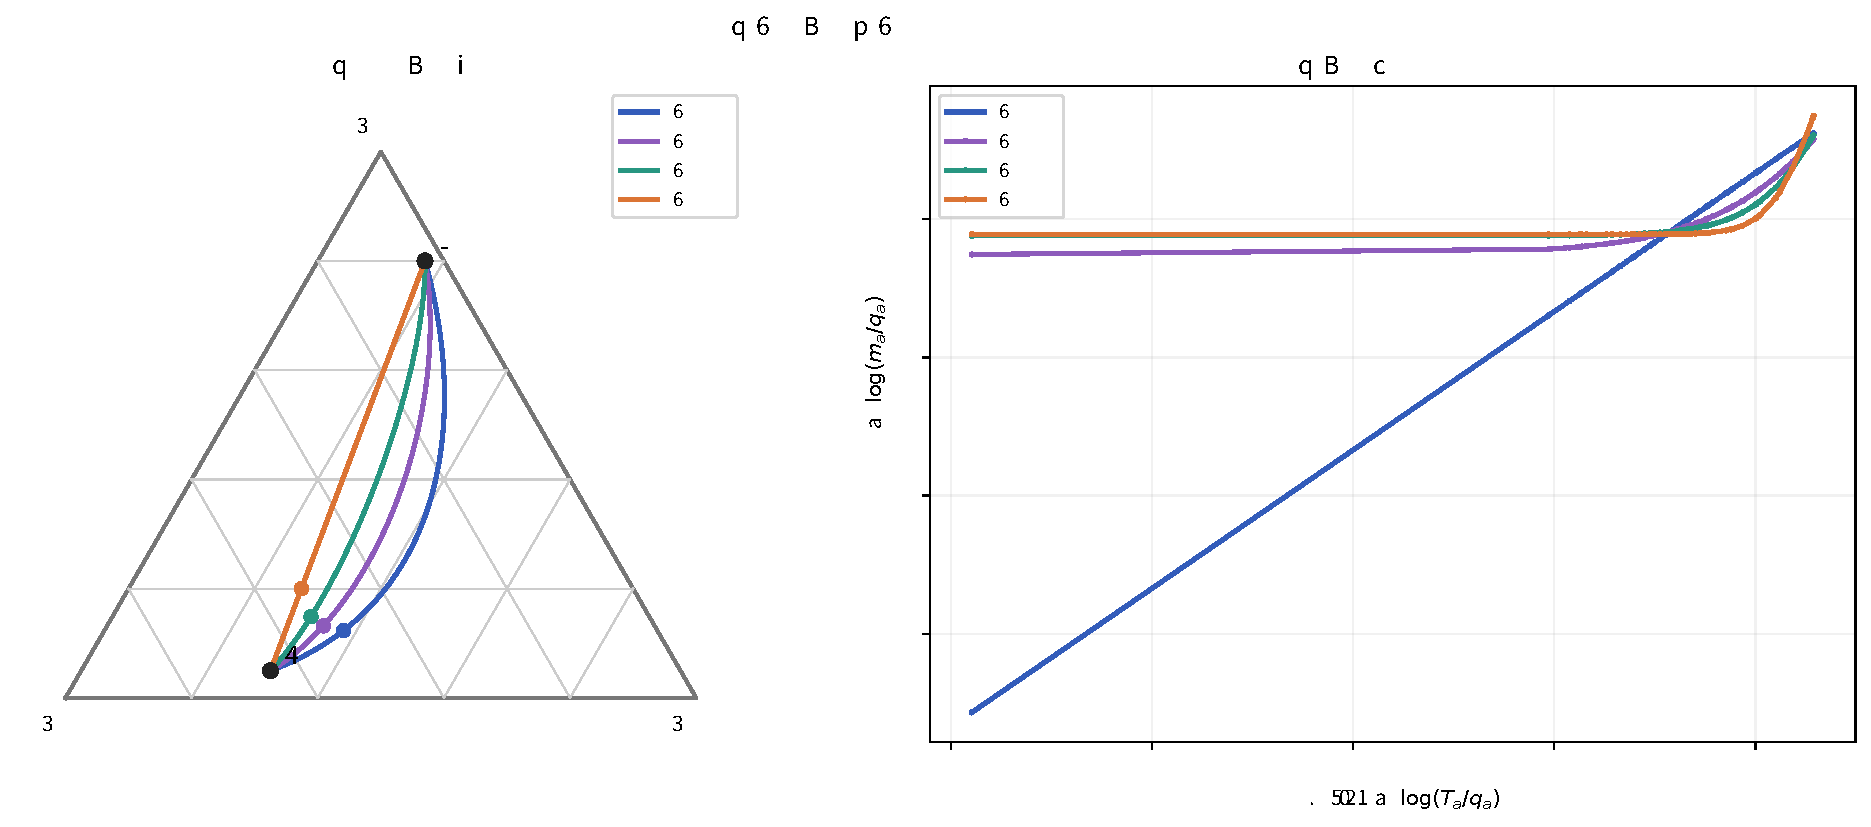
\includegraphics[width=\textwidth]{../../results/proximal-family-geometry/geometry.pdf}
 \caption{幂均值 target 的概率路径与 token log-ratio。左图圆点均为 $\lambda=0.2$；右图以 64 维概率向量展示同一族。形状参数改变高维路径和尾部，而不是仅改变移动距离。}
\end{figure}

\subsection{重心唯一性与超额损失的精确分解}

对 $0<\kappa<1$ 定义
\begin{equation}
 D_\kappa(u\Vert p)
 =\frac{1-\sum_au_a^\kappa p_a^{1-\kappa}}{\kappa(1-\kappa)}.
 \label{eq:proximal-power-divergence}
\end{equation}
Hölder 不等式保证非负，完整支持下等号仅在 $u=p$ 成立。端点由展开给出：当 $\kappa\to0$，$\sum p_a\exp(\kappa\log(u_a/p_a))=1-\kappa\KL(p\Vert u)+O(\kappa^2)$；当 $\kappa=1-\delta\to1$，$\sum u_a\exp(\delta\log(p_a/u_a))=1-\delta\KL(u\Vert p)+O(\delta^2)$。所以
\begin{equation}
 D_0(u\Vert p)=\KL(p\Vert u),\qquad D_1(u\Vert p)=\KL(u\Vert p).
\end{equation}
这固定了本节的 KL 方向，不用不同文献的 $\alpha$ 记号替代定义。

\begin{theorem}[幂均值重心与精确目标误差]
\label{thm:proximal-barycenter-gap}
对 $0<\kappa<1$，令
\begin{equation}
 F(p)=(1-\lambda)D_\kappa(q\Vert p)+\lambda D_\kappa(t\Vert p).
 \label{eq:proximal-divergence-barycenter}
\end{equation}
其唯一最小点是式~\eqref{eq:proximal-power-target} 的 $m$。对任意 $p$ 有
\begin{equation}
 F(p)=\frac{1-Z^\kappa}{\kappa(1-\kappa)}+Z^\kappa D_\kappa(m\Vert p),\qquad
 F(p)-F(m)=Z^\kappa D_\kappa(m\Vert p).
 \label{eq:proximal-gap-identity}
\end{equation}
端点 $\kappa=0,1$ 的超额损失分别为 $\KL(p\Vert m)$ 与 $\KL(m\Vert p)$。
\end{theorem}

\begin{proof}
令 $S_a=(1-\lambda)q_a^\kappa+\lambda t_a^\kappa$。目标写成 $F(p)=(1-\sum_aS_ap_a^{1-\kappa})/[\kappa(1-\kappa)]$。在 $\sum p_a=1$ 约束下，一阶条件为
\begin{equation}
 -\frac{S_a}{\kappa}p_a^{-\kappa}+\nu=0,
 \qquad p_a=(S_a/(\kappa\nu))^{1/\kappa}.
\end{equation}
归一化得到 $m$。目标的概率坐标 Hessian 为 $\operatorname{diag}(S_ap_a^{-\kappa-1})\succ0$，故内点解唯一。由 $S_a=Z^\kappa m_a^\kappa$，直接代入可得
\begin{align}
 F(p)
 &=\frac{1-Z^\kappa\sum_am_a^\kappa p_a^{1-\kappa}}{\kappa(1-\kappa)}\\
 &=\frac{1-Z^\kappa}{\kappa(1-\kappa)}
 +Z^\kappa\frac{1-\sum_am_a^\kappa p_a^{1-\kappa}}{\kappa(1-\kappa)}.
\end{align}
$p=m$ 时散度为零，得精确分解。$\kappa=0$ 时加权 reverse KL 展开为 $\KL(p\Vert m)-\log Z_0$；$\kappa=1$ 时加权 forward KL 展开为 $\KL(m\Vert p)+(1-\lambda)\KL(q\Vert m)+\lambda\KL(t\Vert m)$，其中 $Z_0=\sum q^{1-\lambda}t^\lambda$。端点的超额损失结论随之成立。\hfill$\square$
\end{proof}

定理把“相同 target”加强成了“原重心问题的超额损失与拟合散度精确成比例”。它也给出有限 inner 阶段适合验收的误差：若原问题优化误差为 $\delta$，则 $D_\kappa(m\Vert p)=\delta/Z^\kappa$。MDPO 使用的 $\KL(p\Vert m)$ 与它只有在 $\kappa=0$ 时完全相同；一般 $\kappa$ 下不能仅凭相同最小点替换有限步进展保证。

\subsection{共同的局部 Fisher 曲率与多教师扩展}

取 $p=u+\delta$、$\sum_a\delta_a=0$，并令 $\max_a|\delta_a/u_a|\to0$。逐项展开得到
\begin{equation}
 u_a^\kappa(u_a+\delta_a)^{1-\kappa}
 =u_a+(1-\kappa)\delta_a-\frac{\kappa(1-\kappa)}2\frac{\delta_a^2}{u_a}
 +O(|\delta_a|^3/u_a^2).
\end{equation}
求和后一次项消失，所以 $D_\kappa(u\Vert u+\delta)=\tfrac12\sum_a\delta_a^2/u_a+O(\sum_a|\delta_a|^3/u_a^2)$。在最优点 $m$，$S_am_a^{-\kappa-1}=Z^\kappa/m_a$。故对切向量 $v$、$\sum_av_a=0$，有
\begin{equation}
 \nabla_p^2F(m)[v,v]=Z^\kappa\sum_a\frac{v_a^2}{m_a}.
\end{equation}
若参数化模型恰好实现 $p_\theta=m$，令 $J_\theta=\partial p_\theta/\partial\theta$，则
\begin{equation}
 \nabla_\theta^2F(p_\theta)\big|_{p_\theta=m}
 =Z^\kappa J_\theta^\top\operatorname{diag}(1/m)J_\theta
 =Z^\kappa\mathcal I_\theta(m).
 \label{eq:proximal-fisher-hessian}
\end{equation}
推导中，$\nabla_pF(m)$ 是常数向量，其与 $\partial_\theta^2p_\theta$ 的乘积因 $\sum_ap_{\theta,a}=1$ 而消失。这个等式只在 target 可实现的最优点成立；远离最优点或有模型投影误差时，Hessian 一般还含额外项，不能宣称参数空间全局凸。

多教师 $t^{(j)}$、权重 $w_j\ge0$、$\sum_jw_j=1$ 时，同一证明给出
\begin{equation}
 \argmin_p\sum_jw_jD_\kappa(t^{(j)}\Vert p)
 \propto\left[\sum_jw_j(t^{(j)})^\kappa\right]^{1/\kappa}.
\end{equation}
完整支持下，几何、平方根与算术的多教师汇合均在同一框架内；可将 anchor 作为其中一个分布。超额损失分解及最优点的 Fisher 曲率也直接延续。

\begin{figure}[htbp]
 \centering
 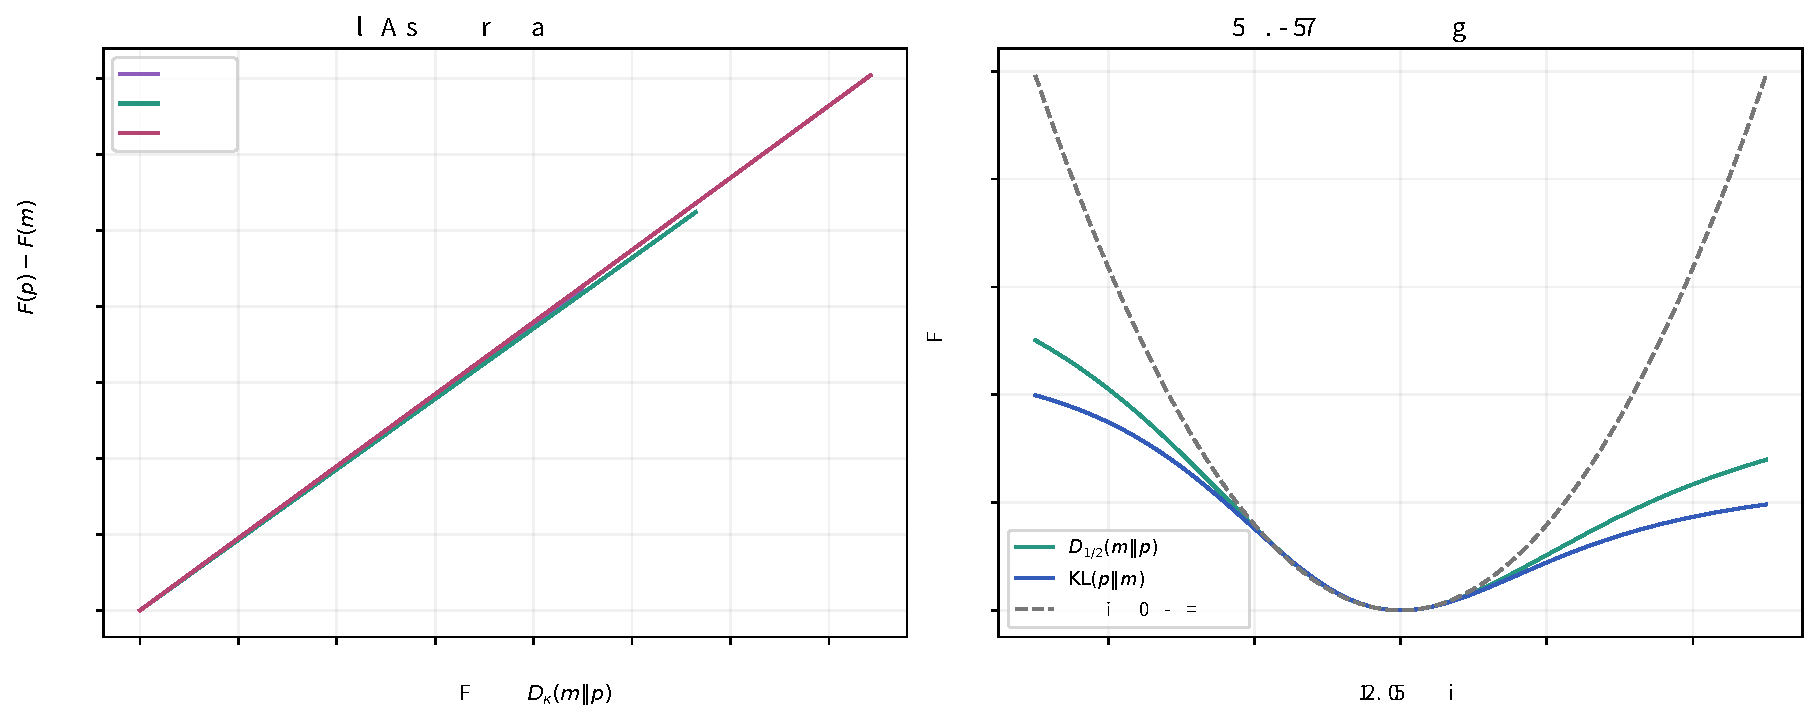
\includegraphics[width=\textwidth]{../../results/proximal-family-geometry/decomposition.pdf}
 \caption{左图检验 $F(p)-F(m)=Z^\kappa D_\kappa(m\Vert p)$，所有点位于对应常数斜率的直线上。右图固定同一个平方根 target，比较 Hellinger 与 reverse KL 拟合：共同的二阶曲率不消除远处损失的差异。}
\end{figure}

\subsection{精确外层与有限 inner 的散度进展}

\begin{theorem}[teacher 散度的进展恒等式]
\label{thm:proximal-teacher-progress}
记 $c_\kappa=Z^\kappa$，端点 $\kappa=0,1$ 取 $c_\kappa=1$。对任意候选 $p$，有
\begin{equation}
 \lambda\left[D_\kappa(t\Vert q)-D_\kappa(t\Vert p)\right]
 =(1-\lambda)D_\kappa(q\Vert p)
 +c_\kappa\left[D_\kappa(m\Vert q)-D_\kappa(m\Vert p)\right].
 \label{eq:proximal-progress-identity}
\end{equation}
若 $D_\kappa(m\Vert p)\le D_\kappa(m\Vert q)$，则 teacher 散度不会增加。精确更新 $p=m$ 且 $q\ne t$ 时严格下降。
\end{theorem}

\begin{proof}
$F(q)=\lambda D_\kappa(t\Vert q)$，而 $F(p)=(1-\lambda)D_\kappa(q\Vert p)+\lambda D_\kappa(t\Vert p)$。由定理~\ref{thm:proximal-barycenter-gap}，$F(q)-F(p)=c_\kappa[D_\kappa(m\Vert q)-D_\kappa(m\Vert p)]$。将 $F(q),F(p)$ 的定义代入并移项，即得恒等式。若目标散度改善，右侧两项非负；若 $p=m$、$q\ne t$，$m\ne q$，则至少第一项严格为正。最后，$m=q$ 会要求 $t_a^\kappa$ 与 $q_a^\kappa$ 成同一比例，概率归一化强制 $t=q$；两个端点同样成立。\hfill$\square$
\end{proof}

这给出了一个纯数学的 finite-inner 条件：降低本轮的 $D_\kappa(m\Vert p)$ 就能提高同一 $D_\kappa$ 下的 teacher 接近度。这里 teacher 散度的方向随 $\kappa$ 改变；一般 $\kappa$ 的保证不能直接替换成每步 $\KL(p\Vert t)$ 都下降。用其他拟合损失获得同一 target，只能在精确求解时自动继承本结论。

\subsection{连续极限是 teacher 散度的自然梯度流}

对 $\lambda\to0$，记 $\rho_a=t_a/q_a$、$A_\kappa=\E_q\rho^\kappa$。逐项展开 $h_a=q_a[1+\lambda(\rho_a^\kappa-1)/\kappa+O(\lambda^2)]$ 并归一化，得到
\begin{equation}
 m_a=q_a+\lambda v_{\kappa,a}+O(\lambda^2),\qquad
 v_{\kappa,a}=\frac{q_a}{\kappa}(\rho_a^\kappa-A_\kappa).
 \label{eq:proximal-natural-velocity}
\end{equation}
展开针对固定完整支持的 $q,t$；其余项不能在任意极端概率比上直接视为统一 $O(\lambda^2)$。$\kappa=0$ 的极限为 $v_{0,a}=q_a[\log\rho_a-\E_q\log\rho]$，$\kappa=1$ 为 $v_1=t-q$。

概率单纯形的 Fisher 度量为 $\langle v,w\rangle_q=\sum_av_aw_a/q_a$。若 $g_a=\partial L/\partial q_a$，则负自然梯度为 $-q_a(g_a-\E_qg)$：其分量和为零，且对任何切向量 $w$，Fisher 内积恰好等于 $-\sum_ag_aw_a$。取 $L(q)=D_\kappa(t\Vert q)$，有 $g_a=-\rho_a^\kappa/\kappa$，因此 $v_\kappa=-\operatorname{grad}_{\!F}D_\kappa(t\Vert q)$。连续时间 $\tau$ 下
\begin{equation}
 \frac{dq_a}{d\tau}=v_{\kappa,a},\qquad
 \frac{d}{d\tau}D_\kappa(t\Vert q)
 =-\|v_\kappa\|_F^2
 =-\frac1{\kappa^2}\Var_q(\rho^\kappa).
 \label{eq:proximal-flow-lyapunov}
\end{equation}
最后一步由 $\sum_av_a=0$ 及 $g^\top v=-(\E_q\rho^{2\kappa}-A_\kappa^2)/\kappa^2$ 得到。$\kappa=0$ 时右侧为 $-\Var_q(\log\rho)$。所有形状参数都对应同一 Fisher 度量，但所下降的全局 teacher 散度不同。

\subsection{escort 坐标中的线性轨迹与全局收敛}

对 $\kappa>0$ 定义 escort 分布和幂和
\begin{equation}
 E_\kappa(q)_a=\frac{q_a^\kappa}{S_\kappa(q)},\qquad
 S_\kappa(q)=\sum_aq_a^\kappa.
\end{equation}
$E_\kappa$ 是单纯形上的双射，逆映射为 $q_a\propto E_\kappa(q)_a^{1/\kappa}$。由 $m_a^\kappa=S_a/Z^\kappa$，共同的归一化因子在 escort 中消失，故
\begin{equation}
 E_\kappa(m)=(1-a)E_\kappa(q)+aE_\kappa(t),\qquad
 a=\frac{\lambda S_\kappa(t)}{(1-\lambda)S_\kappa(q)+\lambda S_\kappa(t)}.
 \label{eq:proximal-escort-step}
\end{equation}
这是精确式，不是局部近似。$\kappa=1$ 时 $S_1=1$，恢复 $a=\lambda$；$0<\kappa<1$ 时，$S_\kappa(q)=\exp((1-\kappa)H_\kappa(q))$，其中 $H_\kappa$ 是 Rényi 熵。因此固定的概率幂插值强度在 escort 坐标中表现为随分布熵改变的有效步幅。

\begin{figure}[htbp]
 \centering
 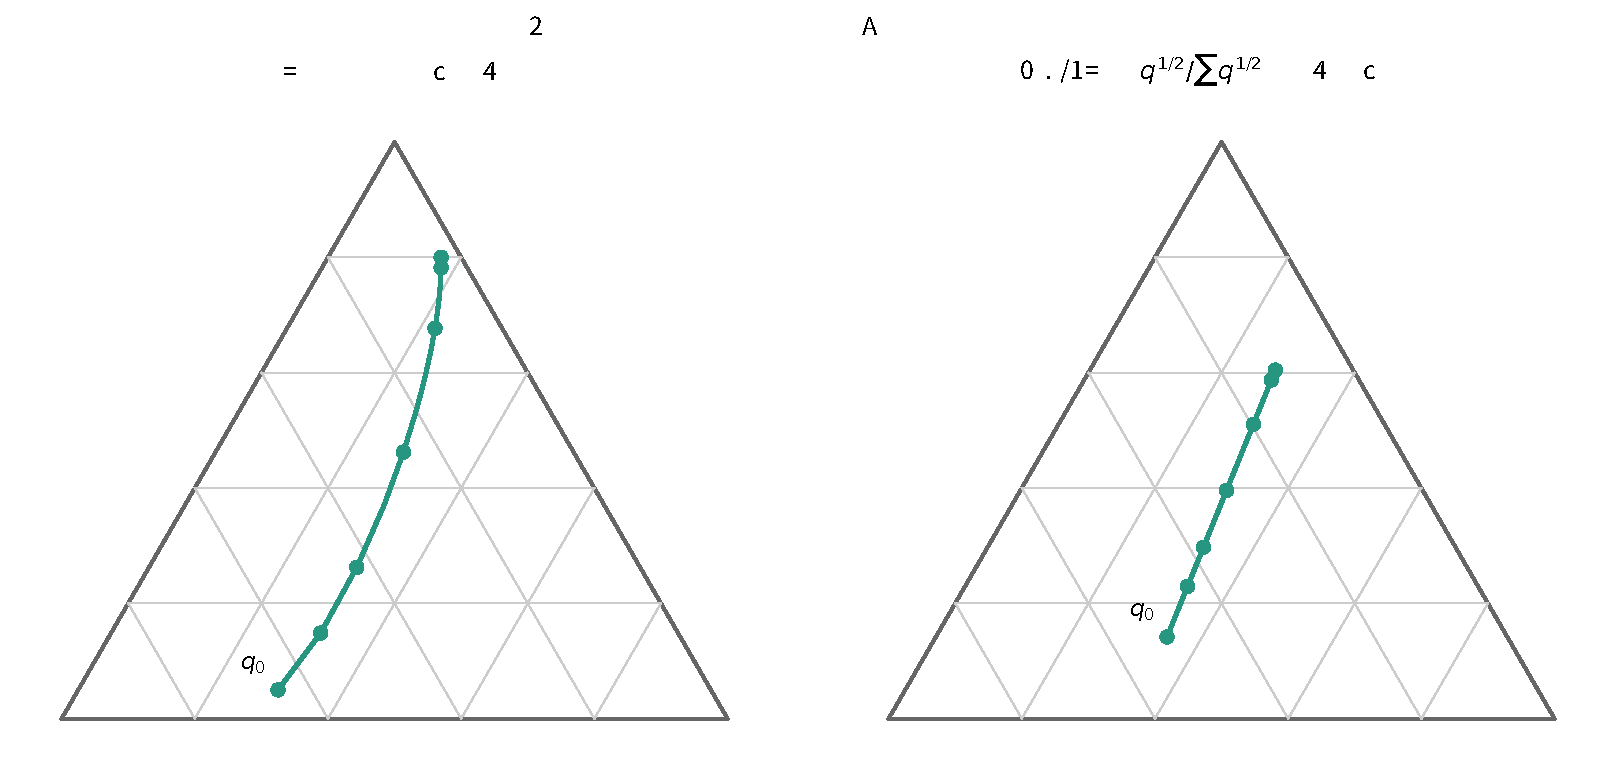
\includegraphics[width=\textwidth]{../../results/proximal-family-geometry/escort.pdf}
 \caption{同一平方根外层轨迹在概率坐标中弯曲，在 escort 坐标中是直线。圆点和数字表示迭代时点。高维分量在固定教师下共享一个进度系数。}
\end{figure}

若 $q_{k+1}=m_{\kappa,\lambda}(q_k,t)$，记 $e_k=E_\kappa(q_k)$，则
\begin{equation}
 e_k-e_t=b_k(e_0-e_t),\qquad
 b_k=\prod_{j=0}^{k-1}(1-a_j).
 \label{eq:proximal-escort-orbit}
\end{equation}
这将固定教师下的 $d-1$ 维精确外层轨迹归结为一个标量 $b_k$。对连续自然梯度流，$dq_a/d\tau=q_a(\rho_a^\kappa-A_\kappa)/\kappa$，所以
\begin{align}
 \frac{d}{d\tau}q_a^\kappa&=t_a^\kappa-A_\kappa q_a^\kappa,\\
 \frac{d}{d\tau}S_\kappa(q)&=S_\kappa(t)-A_\kappa S_\kappa(q),\\
 \frac{d}{d\tau}E_\kappa(q)&=\frac{S_\kappa(t)}{S_\kappa(q)}[E_\kappa(t)-E_\kappa(q)].
\end{align}
改用时间 $\sigma$，$d\sigma/d\tau=S_\kappa(t)/S_\kappa(q)>0$，就有 $e(\sigma)=e_t+e^{-\sigma}(e_0-e_t)$。离散步式~\eqref{eq:proximal-escort-step} 也位于同一条流轨迹上，对应时间增量 $-\log(1-a)$。精确幂均值步因此是这个自然梯度流轨迹的一种时间重参数化，而不只是具有相同起始切线。

\begin{theorem}[teacher 定向的 escort 收缩与误差累积]
\label{thm:proximal-escort-contraction}
令 $d$ 为词表大小，$0<\kappa\le1$，定义度量 $d_\kappa(q,t)=\|E_\kappa(q)-E_\kappa(t)\|_1$。对固定 teacher 的精确更新有
\begin{equation}
 d_\kappa(q_{k+1},t)=(1-a_k)d_\kappa(q_k,t)\le c\,d_\kappa(q_k,t),\quad
 c=\frac{(1-\lambda)d^{1-\kappa}}{(1-\lambda)d^{1-\kappa}+\lambda S_\kappa(t)}<1.
\end{equation}
故 $q_k\to t$。若近似更新满足 $d_\kappa(q_{k+1},m(q_k,t))\le\epsilon_k$，则
\begin{equation}
 d_\kappa(q_k,t)\le c^kd_\kappa(q_0,t)+\sum_{j=0}^{k-1}c^{k-1-j}\epsilon_j,
 \qquad
 \limsup_kd_\kappa(q_k,t)\le\frac{\epsilon_\infty}{1-c}
\end{equation}
其中最后一式要求 $\limsup_k\epsilon_k\le\epsilon_\infty$。
\end{theorem}

\begin{proof}
式~\eqref{eq:proximal-escort-step} 给出距离的精确比例。Jensen 不等式给出 $S_\kappa(q)\le d^{1-\kappa}$，因此 $1-a_k\le c$。反复应用得到精确更新的 $c^k$ 界；escort 逆映射连续，故 $q_k\to t$。近似更新时，三角不等式给出 $d_\kappa(q_{k+1},t)\le\epsilon_k+c\,d_\kappa(q_k,t)$，展开得到有限步式。对任意 $\delta>0$，取 $N$ 使 $j\ge N$ 时 $\epsilon_j\le\epsilon_\infty+\delta$。有限个早期项乘以 $c^{k-1-j}$ 后趋于零，后期项的和不超过 $(\epsilon_\infty+\delta)\sum_{i\ge0}c^i$。令 $\delta\to0$ 得极限上界。\hfill$\square$
\end{proof}

这是对固定 teacher 的定向收缩，不声称两个任意 anchor 经同一算子后具有同一个收缩系数；它也不直接等于原概率空间的 TV 收缩。$\kappa\to0$ 时，escort 本身趋于均匀分布，必须重标度才保留信息：
\begin{equation}
 \frac d\kappa\left[E_\kappa(q)_a-\frac1d\right]
 \longrightarrow\log q_a-\frac1d\sum_b\log q_b.
\end{equation}
几何端点就在这些中心化 log 坐标中满足精确比例 $1-\lambda$。在任何固定完整支持的 teacher 附近，所有 $\kappa$ 都有 $m(t+\delta,t)=t+(1-\lambda)\delta+O(\|\delta\|^2)$，因为 $a_k\to\lambda$。它们共享局部收敛率，远处的度量和有效时间则不同。

\begin{figure}[htbp]
 \centering
 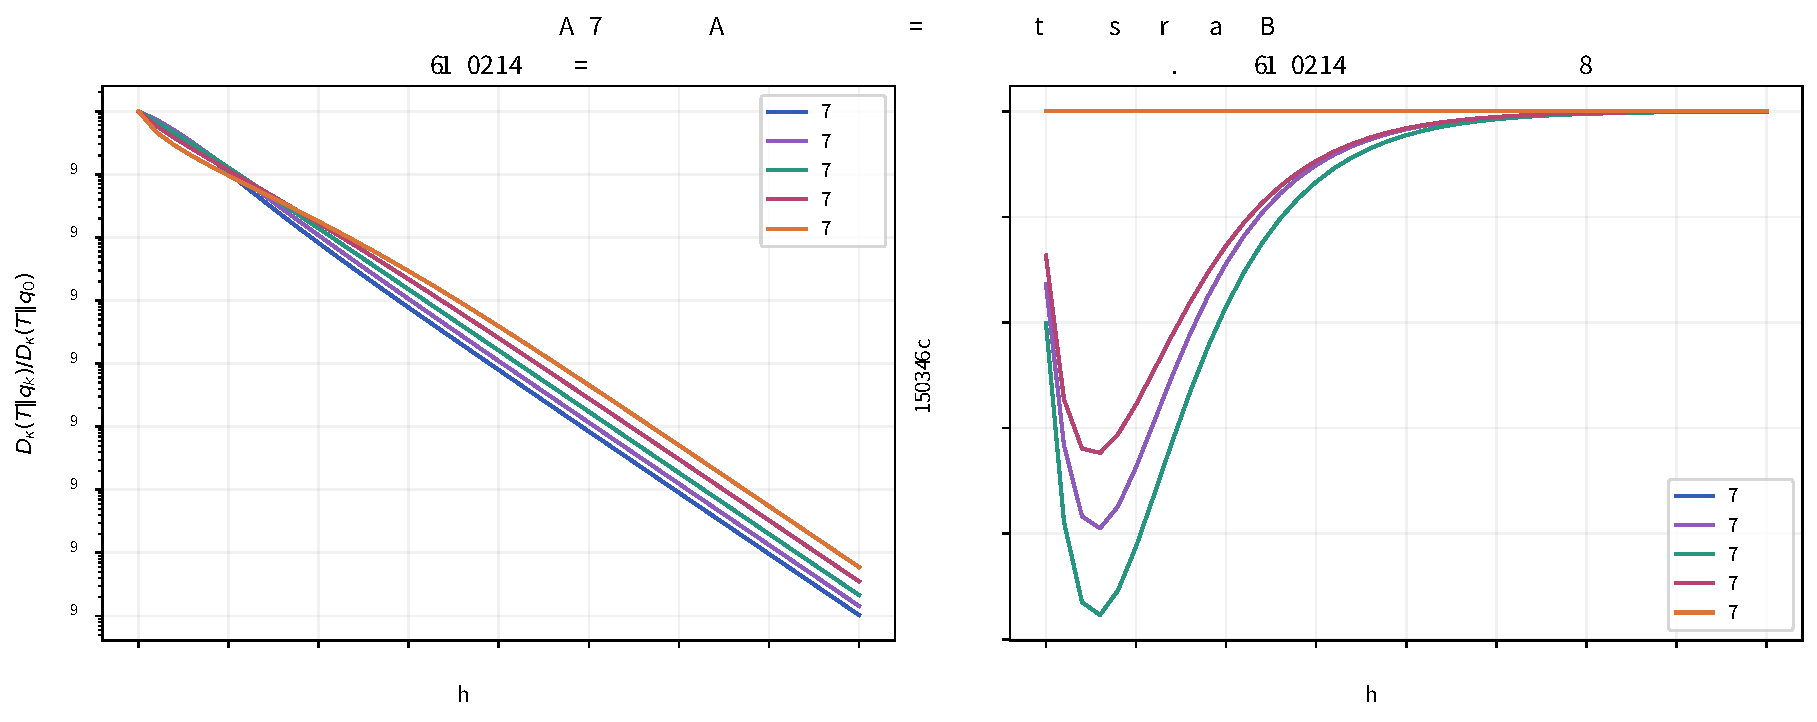
\includegraphics[width=\textwidth]{../../results/proximal-family-geometry/convergence.pdf}
 \caption{精确外层的 teacher 散度单调下降，有效 escort 步幅趋于共同的 $\lambda$。每条曲线使用各自的 $D_\kappa$ 并按初值归一化，图中的高低不能直接作为同一任务的训练性能排名。}
\end{figure}
